\documentclass[tikz]{standalone}
\usepackage{palatino}
\begin{document}
	\begin{tikzpicture}[font=\normalsize]
		\node[anchor=south west,inner sep=0] (image) at (0,0) {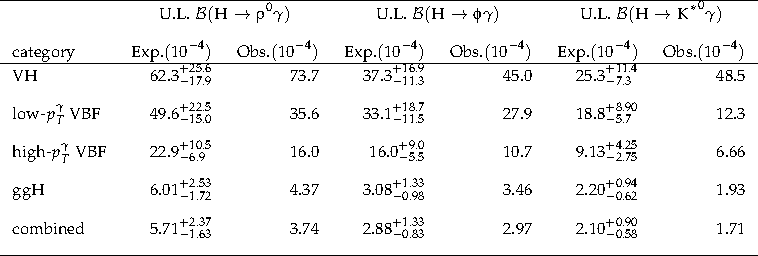
\includegraphics[width=\textwidth]{../23-005-v07-tables/table2.pdf}};
		\begin{scope}[x={(image.south east)},y={(image.north west)}]
			\draw[red,ultra thick] (-0.006,-0.144) rectangle (1.005,1.013);
			\draw[red,ultra thick] (-0.006,-0.144) rectangle (0.242,-0.02);
			\draw (-0.004,-0.146) node[anchor=south west] {\textcolor{red}{\textbf{PAPER (Table 2)}}};
		\end{scope}
	\end{tikzpicture}
\end{document}